\documentclass[tikz, convert={outfile=\jobname.svg}]{standalone}
\usetikzlibrary{positioning}
\begin{document}
\definecolor{cmap1}{HTML}{1f77b4}
\definecolor{cmap2}{HTML}{ff7f0e}
\centering
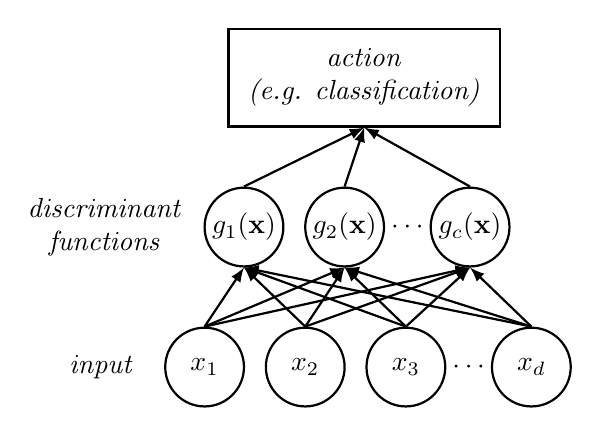
\begin{tikzpicture}[every node/.style={inner sep=0cm, node distance=.25, thick, text opacity=1}]
    \node (action) [rectangle, draw=black, align=center, inner sep=0.25cm, anchor=north]{
        \textit{action} \\ \textit{(e.g. classification)}
    };
    \node (g2) [below = of action, yshift=-0.5cm, xshift=-0.25cm, circle, draw=black, text centered, minimum size=1cm]{
        $g_{2}(\mathbf{x})$
    };
    \node (g1) [left = of g2, circle, draw=black, text centered, minimum size=1cm]{
        $g_{1}(\mathbf{x})$
    };
    \node (discfunc) [left=of g1, rectangle, align=center]{
        \textit{discriminant} \\ \textit{functions}
    };
    \node (gdots) [right=of g2, circle, text centered, minimum size=0cm, xshift=-0.2cm, node distance=0.1cm]{
        $\cdots$
    };
    \node (gc) [right=of gdots, circle, draw=black, text centered, xshift=-0.2cm, minimum size=1cm]{
        $g_{c}(\mathbf{x})$
    };

    \node (x2) [below=of g2, xshift=-0.5cm, yshift=-0.5cm, circle, draw=black, text centered, minimum size=1cm]{
        $x_{2}$
    };
    
    \node (x1) [left=of x2, circle, draw=black, text centered, minimum size=1cm]{
        $x_{1}$
    };
    \node (input) [left=of x1, rectangle, align=center]{
        \textit{input}
    };
    
    \node (x3) [right=of x2, circle, draw=black, text centered, minimum size=1cm]{
        $x_{3}$
    };
    \node (xdots) [right=of x3, circle, text centered, minimum size=0cm, xshift=-0.2cm, node distance=0.1cm]{
        $\cdots$
    };
    \node (xd) [right=of xdots, circle, draw=black, text centered, xshift=-0.2cm, minimum size=1cm]{
        $x_{d}$
    };

    \path[-latex, thick, draw=black] (g1.north) -- (action.south);
    \path[-latex, thick, draw=black] (g2.north) -- (action.south);
    \path[-latex, thick, draw=black] (gc.north) -- (action.south);

    \path[-latex, thick, draw=black] (x1.north) -- (g1.south);
    \path[-latex, thick, draw=black] (x1.north) -- (g2.south);
    \path[-latex, thick, draw=black] (x1.north) -- (gc.south);

    \path[-latex, thick, draw=black] (x2.north) -- (g1.south);
    \path[-latex, thick, draw=black] (x2.north) -- (g2.south);
    \path[-latex, thick, draw=black] (x2.north) -- (gc.south);

    \path[-latex, thick, draw=black] (x3.north) -- (g1.south);
    \path[-latex, thick, draw=black] (x3.north) -- (g2.south);
    \path[-latex, thick, draw=black] (x3.north) -- (gc.south);

    \draw[-latex, thick, draw=black] (xd.north) -- (g1.south);
    \draw[-latex, thick, draw=black] (xd.north) -- (g2.south);
    \draw[-latex, thick, draw=black] (xd.north) -- (gc.south);
\end{tikzpicture}
\end{document}